%%%%%%%%%%%%%%%%%%%%%%%%%%%%%%%%%%%%%%%%%%%%%%%%%%%%%%%%%%%%%%%%%%%%%%%%%%%%%%%%
%2345678901234567890123456789012345678901234567890123456789012345678901234567890
%        1         2         3         4         5         6         7         8

\documentclass[letterpaper, 10 pt, conference]{IEEEtran}  % Comment this line out if you need a4paper

%\documentclass[a4paper, 10pt, conference]{ieeeconf}      % Use this line for a4 paper

\DeclareRelationFont{JY1}{mc}{it}{}{OT1}{cmr}{it}{}
\DeclareRelationFont{JT1}{mc}{it}{}{OT1}{cmr}{it}{}
\DeclareFontShape{JY1}{mc}{m}{it}{<5> <6> <7> <8> <9> <10> sgen*min
    <10.95><12><14.4><17.28><20.74><24.88> min10
    <-> min10}{}
\DeclareFontShape{JT1}{mc}{m}{it}{<5> <6> <7> <8> <9> <10> sgen*tmin
    <10.95><12><14.4><17.28><20.74><24.88> tmin10
    <-> tmin10}{}
\DeclareRelationFont{JY1}{mc}{sl}{}{OT1}{cmr}{sl}{}
\DeclareRelationFont{JT1}{mc}{sl}{}{OT1}{cmr}{sl}{}
\DeclareFontShape{JY1}{mc}{m}{sl}{<5> <6> <7> <8> <9> <10> sgen*min
    <10.95><12><14.4><17.28><20.74><24.88> min10
    <-> min10}{}
\DeclareFontShape{JT1}{mc}{m}{sl}{<5> <6> <7> <8> <9> <10> sgen*tmin
    <10.95><12><14.4><17.28><20.74><24.88> tmin10
    <-> tmin10}{}
\DeclareRelationFont{JY1}{mc}{sc}{}{OT1}{cmr}{sc}{}
\DeclareRelationFont{JT1}{mc}{sc}{}{OT1}{cmr}{sc}{}
\DeclareFontShape{JY1}{mc}{m}{sc}{<5> <6> <7> <8> <9> <10> sgen*min
    <10.95><12><14.4><17.28><20.74><24.88> min10
    <-> min10}{}
\DeclareFontShape{JT1}{mc}{m}{sc}{<5> <6> <7> <8> <9> <10> sgen*tmin
    <10.95><12><14.4><17.28><20.74><24.88> tmin10
    <-> tmin10}{}
\DeclareFontShape{JY1}{mc}{m}{it}{<5> <6> <7> <8> <9> <10> sgen*tmin
    <10.95><12><14.4><17.28><20.74><24.88> tmin10
    <-> tmin10}{}
\DeclareFontShape{JY1}{mc}{bx}{it}{<5> <6> <7> <8> <9> <10> sgen*tmin
    <10.95><12><14.4><17.28><20.74><24.88> tmin10
    <-> tmin10}{}
\DeclareFontShape{JT1}{mc}{m}{it}{<5> <6> <7> <8> <9> <10> sgen*tmin
    <10.95><12><14.4><17.28><20.74><24.88> tmin10
    <-> tmin10}{}
\DeclareFontShape{JY1}{mc}{m}{it}{<5> <6> <7> <8> <9> <10> sgen*tmin
    <10.95><12><14.4><17.28><20.74><24.88> tmin10
    <-> tmin10}{}
\DeclareFontShape{JT1}{mc}{bx}{it}{<5> <6> <7> <8> <9> <10> sgen*tmin
    <10.95><12><14.4><17.28><20.74><24.88> tmin10
    <-> tmin10}{}
\DeclareFontShape{JY1}{mc}{bx}{it}{<5> <6> <7> <8> <9> <10> sgen*tmin
    <10.95><12><14.4><17.28><20.74><24.88> tmin10
    <-> tmin10}{}
\DeclareRelationFont{JY1}{gt}{it}{}{OT1}{cmbx}{it}{}
\DeclareRelationFont{JT1}{gt}{it}{}{OT1}{cmbx}{it}{}
\DeclareFontShape{JY1}{mc}{bx}{it}{<5> <6> <7> <8> <9> <10> sgen*goth
    <10.95><12><14.4><17.28><20.74><24.88> goth10
    <-> goth10}{}
\DeclareFontShape{JT1}{mc}{bx}{it}{<5> <6> <7> <8> <9> <10> sgen*tgoth
    <10.95><12><14.4><17.28><20.74><24.88> tgoth10
    <-> tgoth10}{}
\DeclareRelationFont{JY1}{gt}{sl}{}{OT1}{cmbx}{sl}{}
\DeclareRelationFont{JT1}{gt}{sl}{}{OT1}{cmbx}{sl}{}
\DeclareFontShape{JY1}{mc}{bx}{sl}{<5> <6> <7> <8> <9> <10> sgen*goth
    <10.95><12><14.4><17.28><20.74><24.88> goth10
    <-> goth10}{}
\DeclareFontShape{JT1}{mc}{bx}{sl}{<5> <6> <7> <8> <9> <10> sgen*tgoth
    <10.95><12><14.4><17.28><20.74><24.88> tgoth10
    <-> tgoth10}{}
\DeclareRelationFont{JY1}{gt}{sc}{}{OT1}{cmbx}{sc}{}
\DeclareRelationFont{JT1}{gt}{sc}{}{OT1}{cmbx}{sc}{}
\DeclareFontShape{JY1}{mc}{bx}{sc}{<5> <6> <7> <8> <9> <10> sgen*goth
    <10.95><12><14.4><17.28><20.74><24.88> goth10
    <-> goth10}{}
\DeclareFontShape{JT1}{mc}{bx}{sc}{<5> <6> <7> <8> <9> <10> sgen*tgoth
    <10.95><12><14.4><17.28><20.74><24.88> tgoth10
    <-> tgoth10}{}
\DeclareRelationFont{JY1}{gt}{it}{}{OT1}{cmr}{it}{}
\DeclareRelationFont{JT1}{gt}{it}{}{OT1}{cmr}{it}{}
\DeclareFontShape{JY1}{gt}{m}{it}{<5> <6> <7> <8> <9> <10> sgen*goth
    <10.95><12><14.4><17.28><20.74><24.88> goth10
    <-> goth10}{}
\DeclareFontShape{JT1}{gt}{m}{it}{<5> <6> <7> <8> <9> <10> sgen*tgoth
    <10.95><12><14.4><17.28><20.74><24.88> tgoth10
    <-> tgoth10}{}
\endinput
%%%% end of jdummy.def


\IEEEoverridecommandlockouts                              % This command is only needed if 
                                                          % you want to use the \thanks command

%\overrideIEEEmargins                                      % Needed to meet printer requirements.

% See the \addtolength command later in the file to balance the column lengths
% on the last page of the document

% The following packages can be found on http:\\www.ctan.org
\usepackage{graphics} % for pdf, bitmapped graphics files
\usepackage{epsfig} % for postscript graphics files
\usepackage{mathptmx} % assumes new font selection scheme installed
\usepackage{times} % assumes new font selection scheme installed
\usepackage{amsmath} % assumes amsmath package installed
\usepackage{amssymb}  % assumes amsmath package installed
\usepackage{robomech} 
\usepackage{cite}

\title{\LARGE \bf
Extraction of Precise Spatiotemporal Tactile-Motion Patterns \\ 
in In-hand Manipulation using Sensing Glove
}

\author{Ryo Wakatabe, Yasunori Yamada, Takashi Sagisaka, Yoshiyuki Ohmura and Yasuo Kuniyoshi% <-this % stops a space
%\thanks{*This work was not supported by any organization}% <-this % stops a space
    \thanks{R. Wakatabe, Y. Yamada, T. Sagisaka, Y. Ohmura is Y. Kuniyoshi are with the department of Mechano-Informatics, The University of Tokyo, 7-3-1 Hongo, Bunkyo, Tokyo.  {\tt\small \{wakatabe, y-yamada, sagisaka, ohmura, kuniyosh\}@isi.imi.i.u-tokyo.ac.jp}}%
}

\begin{document}

\maketitle
\thispagestyle{empty}
\pagestyle{empty}

%%%%%%%%%%%%%%%%%%%%%%%%%%%%%%%%%%%%%%%%%%%%%%%%%%%%%%%%%%%%%%%%%%%%%%%%%%%%%%%%
\begin{abstract}
% 一般的なこと
To investigate human manipulation, researchers have measured tactile inputs and motions of the human hand.
% 背景
Tactile measurement of a precision grip by recording tactile nerves have revealed detailed temporal relationship between tacile afferents and gripping force. Recently, sensing gloves enables us to measure manipulations with the whole hand. However, analyses of sensing gloves with higher spatial resolutions can improve the range of observation.
% これは今までの粗い解析では捉えられない接触運動調整を抽出
% 人間の局所化された接触運動制御の示唆を初期的に与えた
In this paper using a sensing glove with high spatio-temopral resolutions and analyses to select tactile-motion variables focusing on precision, we extracted precise tactile points (PTPs) and precise motions (PMs) from a rotating cylinder manipulation. The PTPs are selected such that tactile points get active with high repeatability over trials and their active timings have low variance. Also, the PMs are selected such that motions appear with high repeatability over trials and their timings have low variance. As a result, we showed PTPs and PMs are localized both spatially in the hand and temporally in the task. Moreover, we compared patterns of PTPs and PMs extracted by two manipulations of cylinders with different centers of mass, which are with the identical regrasping procedures. We consequently suggest that patterns of PTPs and PMs characterize precise difference of manipulations that are not distinguishable by previous analyses.
%できれば,specificallyに特定できた,まで言いたいんだが…
% 波及効果
%Our analyses may contribute to human-based control of robotic hand performing in-hand manipulations by presenting precise tactile points and motions as a constraint localized in the manipulation.


%Physiological studies have revealed control of precision grip, e.g., finger force is adjusted to the local frictional condition not to slip manipulating object. These approaches, however, cannot apply to whole-hand control due to technical and ethical problems.
%However, analyses of sensing gloves with higher resolutions can improve the range of observation.
%Recently, development of sensing gloves allows us to analyze whole-hand manipulation. Using the gloves, grasping and manipulation has been categorized to pre-defined few templates.
%In this paper using a sensing glove with high spatio-temopral resolutions, focusing on precision of control, we extracted precise tactile points (PTPs) and precise motions (PMs) from a rotating cylinder manipulation. As a result, we showed PTPs which were active with high repeatability and had low variance of the timimg were localized both spatially in the hand and temporally in the task. In the same way, PMs which extended or bended precisely were spatio-temporally localized in the hand and tha task. Moreover, PTP and PM patterns distinguished two manipulations of rotating cylinders with different center of mass, which are with the identical regrasping procedures. Such precise difference in in-hand manipulations is not distinguishable using previous analyses.
% Such patterns, which can be a constraint of human manipulation using sensing glove, is a useful guideline to design remarkablly dexterous robot hands. 

\end{abstract}


%%%%%%%%%%%%%%%%%%%%%%%%%%%%%%%%%%%%%%%%%%%%%%%%%%%%%%%%%%%%%%%%%%%%%%%%%%%%%%%%
\section{Introduction}
% を以って,人の計測が
%One characteristic of human in-hand manipulation compared to robotic one is the ability to manipulate objects dynamically. To construct robot hands for in-hand manipulation, which and when tactile points and motions are precisely used is important.
%We hypothesized that human hands precisely manipulate neither anytime nor anywhere but spatiotemporally localized. Extracting such localized control enables robots to perform roughly in easy domain and severely in hard one.

% よもやまばなし
% 人の手の運動はダイナミックですごい.でも制御を解析的に求めるのは無理.一方,人はできているので,その接触運動を参考すれば制御できるかもしれない.こういうあぷろーちは大事.
% キーワード 高い接触運動スキル,グラスプだけに留まらない,重要な接触運動の時空間分布,人計測のロボットへの応用
How to control in-hand manipulation with a multi-fingered robotic hand remains a major theme in robotics. Althogh a controller for a in-hand manipulation is achieved analytically based on hybrid system theory, this cannot compute control input in real-time\cite{yingjie2005mld}. In contrast, the human hands can manipulate dexterously. To investigate how the human hands manipulate may contribute to a controller of a robotic hand.

% 従来の接触運動の関係
Physiological studies have revealed tactile-motion control in precision grip. The human hands adjust fingertip forces to the local frictional condition detected by tactile mechanorecepters not to slip the manipulating objects\cite{SensorimotorControlOfManipulationJohansson}. Base on the experimental result, Gunji et al. developed a robotic hand with tactile sensors which can grip unknown various weighted objects\cite{slipandgrip}. However, physiological studies have technical and ethical difficulty in measuring a whole hand manipulation because they are based on invasive measurement.

% データグローブで手全体が取れるようになった.
Recently, development of sensing gloves and systems allows us to measure whole hand. Using a sensing glove with 15 tactile sensors, tactile patterns during grasp and place task are categorized to 7 pre-defined grasping templates\cite{Faria}. Also, using 5 tactile groups, a transition of 32 pre-defined grasping patterns is categorized to 6 manipulation templates\cite{Kondo}. However, analyses characterizing manipulations using sensing glove with more tactile points can improve the range of observation. 

% 制御の分散に着目することの重要性
% On the other hand, several researchers analyzes human motion focusing on variance of state. 
% 一方,他の人の運動解析では,state-spaceのダーツいろいろやっている グローバルダイナミクス的さむしん しかし,手に対してやってるのない
Researchers on human motion and robot control have focused on spatial and temporal variance of state-space. Uncontrolled manifold analysis can select coordinating variables in human motion based on spatial variance over trials\cite{nonaka2013motor}. Moreover, when humans and robots perform dynamic whole-body actions (role-and-rise task, for expamle), states-space with small variance sparsely located along the time axis is known to be a critical condition for a control to succeed \cite{kuniyoshi2007emergence}. However, the human hands have not been analyzed from the point of view of variance of state-space.

%%%%%%%%%%%%%%%%%%%%%%%%%%%%%%%%%%%%%%%%%%%%%%%%%%%%%%%%%%%%%%%%%%%%%%%%%%%%%%%%

\section{Materials and Methods}
% 今回使用した実験手順を抽象化して、どのような 状況で使える手法なのか、何がわかるようになる手法なのか、なぜそのような手 法が必要なのか、従来手法とどう違うのか、という観点で書く必要がある。 たとえば、precise tactile pointsというのは、動作に周期性を仮定していると 思うけど、それはIIIの最初に明記すべき。 IIIが提案なので、この節で完結するように、ロジックを記述する必要がある。
% ここ順番がめちゃくちゃ
%It is important for a robot designer to know which tactile points and motions plays crucial role to a in-hand manipulation. One of the ways to extract such tactile points and motions is to measure human in-hand manipulation and analyze its structures. 

%In order to record natural human in-hand manipulation, we require sensing glove with 3 following features: able to measure tactile points and motions simultaneously, thin enough not to inhibit human manipulation and enough to copy human tactile inputs. 

%We hypothesized such tactile points and motions that activates with both spatial and temporal precision because they can be a strong constraint of in-hand manipulation. We considered there are two precision, spatial one and temporal one. First, spatial precision which is defined by repeatability of activation gives us a constraint on which tactile points and motions should be used constantly in a specific in-hand manipulation. Second, temporal precision indicating a variance of activated timing presents a constraint on when tactile points and motions should activate. 

%Using the indicators, repeatability and time variance, we analysed three structures of manipulations: the identical regrasping procedure, spatial distribution of precise tactile points and motions and temporal distribution of them. Regrasping procedure is defined as sequence of movements of fingers. We predicted that precision of tactile points and motions in manipulations were different even when the manipulations had the identical regrasping procedure. In order to make sure the difference among patterns of precise tactile points and motions was derived not by different regrasping procedure but by tactile-motion dynamics. Note that previous research based on clusterizing and grasp taxonomy can not discriminate these two manipulation. 

%If a certain tactile point is shared by a little different two manipulations, it can be fundamental tactile point for the manipulations in common. On the other hand, it is

\subsection{Tactile-Motion Sensing Glove}
We employed tactile-motion sensing glove which has hand motion capture system and physiologically sound dense tactile sensing glove\cite{SagisakaONOK12}. Hand motion capture system is implemented with inertia sensors on the back of the hand in order not to inhibit human manipulation (\figref{fig:glove}(b)). Hand motion capture system has 18 inertia sensors (222 fps). Tactile sensing glove has spatial and temporal resolutions comparative to be comparable to human hand (\figref{fig:glove}(a)). The spatial resolution is based on two-point discrimination of the human hand\cite{weinstein1968intensive}. The glove has approximately 1000 pressure sensors, the number of which depends on size of subject's hand, at 1000 fps. This glove also minimize the inhibitation by being made thin.

\begin{figure}[t!]
 \centering
  \includegraphics[width=0.40\textwidth]{figure/method/tactile-motion-capture-system.eps}
 \caption{Appearance of tactile sensing glove and hand motion capture system.}
 \label{fig:glove}
\end{figure}


\subsection{Precise Tactile Points and Motions}
%(この章全体が不自然.整理して,数学的概念を明確に,適切な用語を使う)
%(重要な概念なのに初出か同じ名前のセクションで厳密明確な定義なし,致命的.PTPなど略語割り当てるべき.)
%(この節全体に言えるが,数式できっちり定義すべき.)
% 具体的な抽出方法

%To extract {\it Precise Tactile Point} (PTP) and {\it Precise Motion} (PM) from human manipulation, we formally define them as follows. We are given $ M $ 
We extracted PTPs and PMs by high repeatability and low time variance over trials (\figref{fig:way-to-extract}). The procedure to extract PTPs and PMs is as follows: (1) We segmented raw time-series to trials by tactile event, e.g., initial contact between a thumb and a manipulating object. (2) We linearly normalized the length of time duration of trials to phase in $[0, 1]$. (3) We extracted tactile point activated for the first time and its timing for each manipulation segment. In the same way, we extracted motions defined as extention and bending for the first time and its timing for each segment. If a motion has 2 or more extention and bendings, we dismissed the motion. (4) If the tactile point which activates more than preset threshold (90\%, here) of all trials and the standard deviation of the timing is less than preset threshold (0.15, here), we extracted them as PTPs. In the same way, if the motions which always extend or bend and the standard deviation of the timing is less than preset threshold (0.15, here), we extracted them as PMs. 

% 空間分布
To investigate spatial distribution of PTPs, we visualized PTPs by plotting on a 3D model of the hand, which was scanned by 3D scanner.  

% 時間分布(ある時間区間におけるover trial)
To examine temporal distribution of PTPs, we used {\it mean active rate} as the index to indicate the instantaneous number of active PTPs. Mean active rate is defined as the mean of the count of active PTPs in an interval of preset duration T (0.09, here). Tactile distribution of PTPs is calculated by the average over trials of mean active rate of PTPs for all phase. To investigate which PTPs are extracted in a specific time section, we visualized repeatability of PTPs activated in the section by plotting on a 3D model of the hand.
%time sectionの定義we defined the section of manipulation by local minima of we used the average of mean active rate of all tactile points over trials because such timing indicates the beginning of touch.


% 抽出方法
\begin{figure}[t!]
 \centering
  \includegraphics[width=.49\textwidth]{figure/method/extraction-of-tacmot.eps}
  \caption{Precise tactile point (PTP) and precise motion (PM). (a) A tactile point that it gets active with high repeatablity and the variance of active timing is low. (b) A precise motor such that it extends or bends with high repeatability and the variance of motion timing is low.}
 \label{fig:way-to-extract}
\end{figure}

%%%%%%%%%%%%%%%%%%%%%%%%%%%%%%%%%%%%%%%%%%%%%%%%%%%%%%%%%%%%%%%%%%%%%%%%%%%%%%%%

\section{Manipulation Experiment}
\subsection{Experimental Setup}
% トライアルの数とsingle-subjectが離れている上に,single-subjectの理由付けなし.
We conducted a single-subject experiment to measure and analyse in-hand manipulation, rotating in-hand manipulation. The subject performed 2 rotating manipulations of cylinder objects with center of mass coinciding with the geometrical center (manipulation C) and biased one (manipulation NC) wearing the sensing glove (\figref{fig:cylinder}, \tabref{tab:specification-of-robot}). The subject was told to just rotate the object on the table in one direction without any instruction of rotating velocity and regrasping procedure. To record natural manipulations, the subject was not told which of the two (C/NC) he was holding. The subject repeatedly rotated the cylinder 17 times in manipulation C and 26 times in manipulation NC. This experiment is conducted under ethical approval and informed consent of the subject.

\begin{figure}[t!]
 \centering
 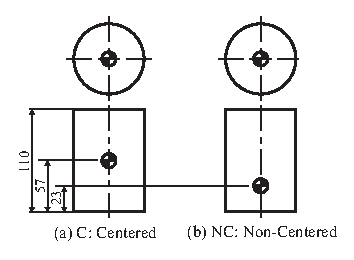
\includegraphics[width=0.3\textwidth]{figure/method/cylinder-property.eps}
 \caption{Manipulated cylinders.} 
 \label{fig:cylinder}
\end{figure}

\begin{table}[t!]
 \centering
 \caption{Specification of the cylinders.}
      \begin{tabular}{|r||l|l|} \hline
               & Manipulation C & Manipulation NC \\ \hline \hline
              Weight & 455 g & 322 g \\ \hline
              Height & 110 mm & 110 mm \\ \hline
              Height of center of gravity & 57 mm & 23 mm \\ \hline
              Diameter & 72 mm & 72 mm \\ \hline
            \end{tabular}
    \label{tab:specification-of-robot}
\end{table}


% 実験風景
\begin{figure}[t!]
  \centering
  \includegraphics[width=0.45\textwidth]{figure/method/experiment-overview.eps}
  \caption{Overview of in-hand manipulation measurement. (A) Overview of experiment. (B) Reconstructed hand state using tactile sensing glove and motion capture system.}
 \label{fig:experiment-overview}
\end{figure}


\subsection{Identical Regrasping Procedure in In-hand Manipulation}

We observed the identical regrasping procedure in both manipulation C and NC (\figref{fig:snapshot}). Observed regrasping procedure is as follows:
\begin{itemize}
    \item[A.] Put the index finger and the fingers from middle to little on the object
    \item[B.] Put the index finger to the object immediatele after rotating the object
    \item[C.] Release and stretch the fingers from miggle to little.
    \item[D.] Regrasp the object with all fingers
    \item[E.] Bend a thumb and put it to the object
\end{itemize}

% 操作のスナップショット
\begin{figure*}[t!]
  \centering
  \includegraphics[width=0.98\textwidth]{figure/method/snapshot-m1.eps}
  \caption{Snapshots of rotating manipulation. The pictures of A-E represent the corresponding regrasping procedure.}
 \label{fig:snapshot}
\end{figure*}

\begin{figure*}[t!]
% 図: 抽出された接触運動
 \centering
  \includegraphics[width=.98\textwidth]{figure/experiment/m-db-ext.eps}
  \caption{Representative raster plots and mean active rate of PTP and non-PTPs from manipulation C and NC. Red points indicate PTPs. Gray points indicate non-PTPs. Blue solid line represents mean active rate of PTPs. Blue dashed line represents mean active rate of all tactile points.}
 \label{fig:m-db-ext}
\end{figure*}

\subsection{Result}
%(全体的に英語の記述の意味がわからない.肝心が結果なのにわからないのは致命的.長々と拙い表現で説明せず,定義した量・グラフ・検定などデータに依ってごく簡潔明瞭に結果を提示すべき)
We characterized manipulation C and NC respectively focusing on the numbers, spatial distributions and temporal distributions of PTPs and PMs. First, the number of PTPs was 99 in manipulation C and 186 in manipulation NC. Similarly, the number of PMs was 2 in manipulation C and 12 in manipulation NC (\figref{fig:comp-tac}B, \figref{fig:comp-mot}). This shows that the in-hand manipulations were characterized not by all tactile points and motions but by partial ones, PTPs and PMs. Second, both PTPs from manipulation C and NC were localized in from a thumb to the ring finger and the palm near a thumb (\figref{fig:tac-dist}). Moreover, The PMs from manipulation C were localized in motions of a thumb. The PMs from manipulation NC were also localized in motions of the fingers except for second finger (\figref{fig:comp-mot}). We found spatial distributions of PTPs and PMs was localized. Third, temporal distrivution of PTPs and PMs was also localized. The representative segment shows that the PTPs from manipulation NC are localized in 3 time sections and the PTPs from manipulation C are localized in 2 time sections. Also, the PMs from manipulation C and NC were localized along the time-axis (\figref{fig:comp-mot}). We therefore found temporal distribution of PTPs and PMs were localized.

% 図: 運動の比較
\begin{figure}[t!]
 \centering
  \includegraphics[width=.48\textwidth]{figure/experiment/mot-comp-with-cap.eps} %{figure/final/motion-time-distribution-trial-1_2.eps} 
 \caption{Temporal distribution of PMs from manipulations of C and NC.}
 \label{fig:comp-mot}
\end{figure}


\begin{figure}[t!]
 \centering
  \includegraphics[width=.48\textwidth]{figure/experiment/tac-distribution.eps}
  \caption{Spatial distribution of PTPs from manipulations C and NC. (A) Spatial distribution of manipulation C. (B) Spatial distribution of manipulation NC.}
 \label{fig:tac-dist}
\end{figure}


To examine the difference of PTPs and PMs between manipulation C and NC, we compared manipulation C and NC focusing on share of spatial distributions and temporal distributions. First, the PTPs extracted from manipulation C shared 70\% (69 points) of these from manipulation NC (\figref{fig:comp-tac}B). The number of the PTPs only from NC was 117 points (11.5\% of the total). Also, all the PMs from manipulation C were extracted from manipulation NC. This suggest that there are common and task-specific PTPs and PMs. Second, we found there was three sections defined by local minima of the all tactile points. In the third section, the PTPs was found only from manipulation NC (see blue sections in \figref{fig:temporal-tactile-points-with-variance}AB). The temporal difference of PTPs were localized in a specific section. Third, visualizing the spatial distribution of the PTPs in each section, we found two spatial differences: on the one hand, PTPs in the third finger and fourth finger was different in the third section (\figref{fig:temporal-tactile-points-with-variance}EH). On the other hand, PTPs in the pulp of the second finger differed in the second section (\figref{fig:temporal-tactile-points-with-variance}DG). We found spatio-temporally localized specific differences of PTPs and PMs.

% 図: 接触運動の包含関係
\begin{figure}[!t]
 \centering
  \includegraphics[width=0.48\textwidth]{figure/experiment/comp-tac-with-cap.eps}
  \caption{Share relationship between PTPs in manipulation C and manipulation NC. (A) Spatial distribution of PTPs in manipulation C and NC. Light red points represent PTPs in manipulations both C and NC, blue points from only from manipulation C, dark red from only from manipulation NC. (B) A Venn diagram of PTPs from manipulations C and NC.}
 \label{fig:comp-tac}
\end{figure}



% 分散付きの空間比較
% TODO figure not yet
\begin{figure*}[t!]
 \centering
  \includegraphics[width=.98\textwidth]{figure/experiment/temporal-tactile-points-with-variance.eps}
%  \includegraphics[width=.48\textwidth]{figure/experiment/temporal-tactile-points-with-variance.eps}
  \caption{Spatio-temporal distribution of PTPs at each section. (A and B) The average over trials of the mean active rate of the tactile points in manipulation C and NC. Red solid line and envelop indicate the average and variance of the mean active rate of PTPs over trials. Black solid line and envelop indicate the average and variance of the mean active rate of all tactile points over trials. (C-E) Spatial distribution of PTPs extracted from manipulation C at each section. (F-H) Spatial distribution of PTPs extracted from manipulation NC at each section.}
 \label{fig:temporal-tactile-points-with-variance}
\end{figure*}


%%%%%%%%%%%%%%%%%%%%%%%%%%%%%%%%%%%%%%%%%%%%%%%%%%%%%%%%%%%%%%%%%%%%%%%%%%%%%%%%
\section{Conclusion and Discussion}
% conclusion
In this paper using a sensing glove with high spatio-temopral resolutions and analyses to select tactile-motion variables focusing on precision, we extracted precise tactile points (PTPs) and precise motions (PMs) from a rotating cylinder manipulation. The PTPs are selected such that tactile points get active with high repeatability over trials and their active timings have low variance. Also, the PMs are selected such that motions appear with high repeatability over trials and their timings have low variance. As a result, we showed PTPs and PMs are localized both spatially in the hand and temporally in the task. Moreover, we compared patterns of PTPs and PMs extracted by two manipulations of cylinders with different centers of mass, which are with the identical regrasping procedures. We consequently suggest that patterns of PTPs and PMs characterize precise difference of manipulations that are not distinguishable by previous analyses.

% 重要だと言われていたが,その方法は確立していない.
% 手で初めて正確な状態を抽出.起き上がりのコツに似ている.従って,in-hand manipulationに新たな光
Although control for dextrous manipulation with robot hand is an important open problem\cite{bicchi2000hands}, there have not been a realistic controller. On the other hand, dynamic whole-body actions including complex contacts with the ground, for example roll-and-rise task, are known to have a "knack", an extremely narrow region in state-space to success\cite{kuniyoshi2007emergence}. The knacks is extracted by measuring human roll-and-rise task based on convergence of the variance of motion trajectories. Focusing on the knacks extracted from human measurement, a real adult-size humanoid robot performs roll-and-rise motion\cite{kuniyoshi2004dynamic}. Similar to dynamic whole-body actions, we consider that PTPs and PMs extracted from human in-hand manipulation enables control of robotic in-hand manipulation.

% 難易度
We show that the human hands adapt to a more difficult manipulation by adding PTPs patterns. Manipulation NC is more difficult than manipulation C because the center of gravity of the cylinder used in manipulation NC is closer to the edge of supprting hand polygon than manipulation C. Focusing on the difference of PTPs patterns, additional spatio-temporal patterns are extracted only from manipulation NC. This implies that more difficlt task requires more additional TPT patterns to stabilize the manipulation.

% 今後(網羅的調査,ダイナミックなマニピュレーションの拘束条件としてロボットの構成)
In future work, we will conduct experiment to extract precise tactile-motion patterns from other in-hand manipulations. On the longer term, we plan to construct a robot controller using precise tactile-motor pattern extracted from human in-hand manipulation.
\addtolength{\textheight}{-12cm}   % This command serves to balance the column lengths
                                  % on the last page of the document manually. It shortens
                                  % the textheight of the last page by a suitable amount.
                                  % This command does not take effect until the next page
                                  % so it should come on the page before the last. Make
                                  % sure that you do not shorten the textheight too much.


%%%%%%%%%%%%%%%%%%%%%%%%%%%%%%%%%%%%%%%%%%%%%%%%%%%%%%%%%%%%%%%%%%%%%%%%%%%%%%%%
%\section*{ACKNOWLEDGMENT}
%We particularly thank Takashi Sagisaka to his incredible sensing glove. We are grateful to Yasunori Yamada to many discussion on the method and his advice on this paper. We thank Yoshiyuki Ohmura to his valuable comments on the maniscript. 

%%%%%%%%%%%%%%%%%%%%%%%%%%%%%%%%%%%%%%%%%%%%%%%%%%%%%%%%%%%%%%%%%%%%%%%%%%%%%%%%

%\begin{thebibliography}{99}
%\bibitem{c1} G. O. Young, Synthetic structure of industrial plastics (Book style with paper title and editor), 	in Plastics, 2nd ed. vol. 3, J. Peters, Ed.  New York: McGraw-Hill, 1964, pp. 1564.
%\end{thebibliography}



\bibliographystyle{IEEEtranS}
%\bibliographystyle{junsrt}
\bibliography{bibTeX/thesis}



\end{document}
